\section{Introduction} \label{sec:introduction}

It is generally agreed upon that large-scale, universal quantum computing will require comprehensive error correction. One often considered error-correcting code is the so-called surface code, but the question remains how to experimentally implement it. In \cite{OGorman2016}, O'Gorman \textit{et al}. proposed a method which relies on physically moving probe qubits across four data qubits to perform the stabiliser measurement. In the paper, they performed a large scale simulation and found reasonable fault-tolerance thresholds which suggest that the proposal is both viable and scalable. 

In this report, we will build upon their proposal and simulate a simple model that contains all the essential features. We will focus on four data qubits and one probe qubit, and introduce individual errors into the simulations to see how the performance of the system is affected. The report is structured as follows: In the subsequent sections, we will introduce the surface code and the results obtained in \citet{OGorman2016}. We will then go on to review the methods used in the simulation in section \@ \ref{sec:simulation} as well as review the spin species available for an eventual experimental implementation. Following that, in section \@ \ref{sec:errors} we introduce errors into our model and show how they affect the performance. Finally, we summarise our results in section \@ \ref{sec:conclusions} and provide a number of suggestions regarding where future investigations can be concentrated. 

A Git repository containing the code used in our work can be found at \url{https://github.com/sqvarfort/data_probe_qubit_simulation}. 

\subsection{The surface code}
The surface code is one of the most-well studied fault-tolerant codes \cite{Wang2011,Fowler2012}. Its versatility, large code distance, and large fault-tolerance threshold ($1.1\%$) have contributed to various proposals \cite{Fowler2012,Pica2014,Tosi2015,Hill2015,OGorman2016} and some attempts at physical implementation \cite{Barends2014,Kelly2015}. One key aspect of the surface code is its use of vertex and plaquette operators that perform stabiliser measurements on all data qubits using ancillary qubits. If one stabiliser gives a measurement outcome $-1$, it means that these specific four data qubits have undergone an error, whereas a $+1$ outcome indicates that the qubit states are in the codespace. As a consequence, the stabiliser measurements cannot identify errors that correspond to logical operations. At the same time, the stabiliser allows us to actually perform logical operations, which means that a physical implementation of the surface code would not require individual addressing of the data qubits, apart from some global initialisation method. 

The stabiliser measurements require several data qubits to interact with one ancillary qubit. This probe qubit is then measured, and its outcome is essentially a parity measurement of the four data qubits, that is, whether none or two  (even parity), or one or three (odd parity) errors have occured. Given the outcome of the measurement, subsequent error correction methods can then be considered. By only measuring the parity of the data qubits, no distinction is made between them and any quantum information is preserved. 






\subsection{A physical implementation} \label{sec:PhysicalImplementation}
As mentioned in section \ref{sec:introduction},  \citet{OGorman2016} proposed a scheme for implementing the surface code in silicon. In this proposal the stabiliser measurements are realised by a mechanical approach, where the data and probe qubit arrays are embedded in two separate layers (see fig.\@ \ref{FIG:paper-mems}). Both layers are brought into close contact ($d\ll D$) and a relative motion of one layer with respect to the other leads to the probe qubits orbiting above the data qubits. This movement allows to perform the stabiliser measurement by realising a parity measurement where one probe qubit interacts with four data qubits throughout its orbit (see fig.\@ \ref{FIG:paper-parity}). Microelectromechanical systems (MEMS) could be used to implement this motion.


\begin{figure}[H]
	\centering
	\subfloat[]{ 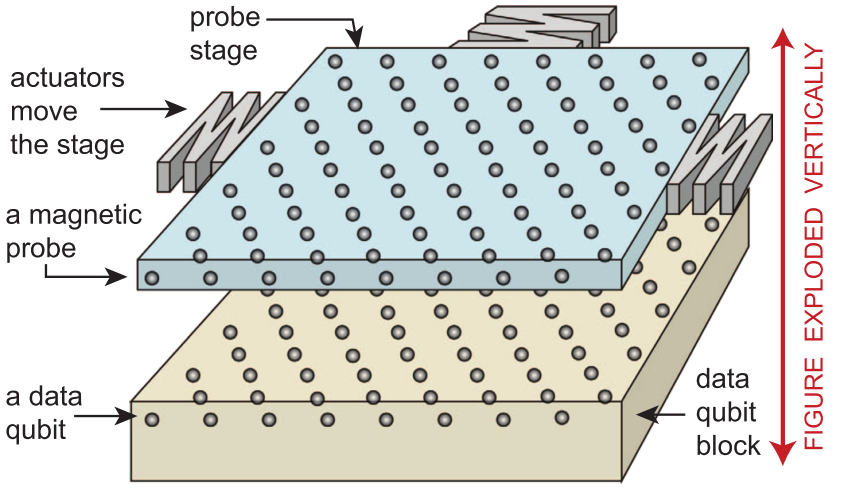
\includegraphics[width=0.8\linewidth]{../Figures/paper-mems} \label{FIG:paper-mems}}\\
	\subfloat[]{ 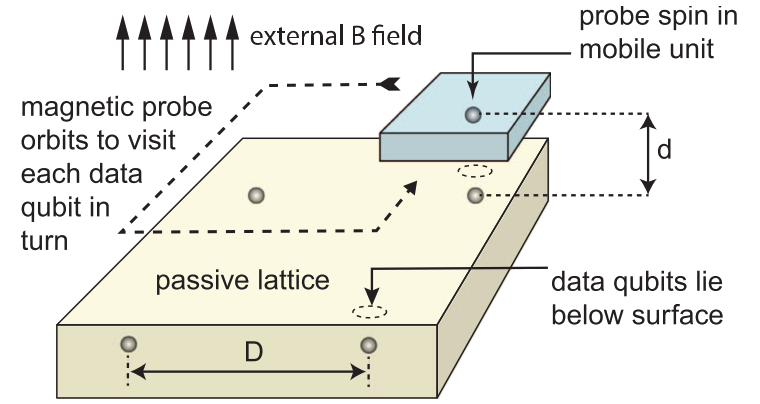
\includegraphics[width=0.8\linewidth]{../Figures/paper-parity} \label{FIG:paper-parity}}
	\caption[paper]{\textbf{(a)} Schematic of a scalable processor where data and ancillary/probe qubits are arranged in arrays in two different layers/stages which are moving relative to each other. \textbf{(b)} Magnified view of four data and one probe qubit. The movement results in the probe qubit orbiting above the data qubits allowing to implement a parity measurement. Direct copy from \cite{OGorman2016}.}
	\label{FIG:paper}
\end{figure}

This scheme requires a high precision in qubit placement. Therefore, \citet{OGorman2016} performed large-scale fault-tolerance simulation to obtain thresholds on the qubit placement precision. The orbit and movement can be performed in many different ways. They presented results for an abrupt orbit, where the probe qubit is moved rapidly from one data qubit to another, and a smooth, circular orbit.

Several thresholds were obtained with respect to the qubit placement precision where the data qubit displacement distribution takes either a `pillbox' (see fig.\@ \ref{fig:pillbox}) or an ellipsoid shape.
They found reasonable thresholds for each configuration compared to current qubit placement precisions offering good prospects for achieving logical qubit protection at the large scale. 

If we were to implement such a system in the lab, we would probably start with the smallest possible building block, which in this case is the system consisting of four data qubits and a single probe qubit to demonstrate a single parity measurement.
